%  LaTeX support: latex@mdpi.com
%  For support, please attach all files needed for compiling as well as the log file, and specify your operating system, LaTeX version, and LaTeX editor.

%=================================================================
% pandoc conditionals added to preserve backwards compatibility with previous versions of rticles

\documentclass[,article,submit,moreauthors,pdftex]{Definitions/mdpi}


%% Some pieces required from the pandoc template
\setlist[itemize]{leftmargin=*,labelsep=5.8mm}
\setlist[enumerate]{leftmargin=*,labelsep=4.9mm}


%--------------------
% Class Options:
%--------------------

%---------
% article
%---------
% The default type of manuscript is "article", but can be replaced by:
% abstract, addendum, article, book, bookreview, briefreport, casereport, comment, commentary, communication, conferenceproceedings, correction, conferencereport, entry, expressionofconcern, extendedabstract, datadescriptor, editorial, essay, erratum, hypothesis, interestingimage, obituary, opinion, projectreport, reply, retraction, review, perspective, protocol, shortnote, studyprotocol, systematicreview, supfile, technicalnote, viewpoint, guidelines, registeredreport, tutorial
% supfile = supplementary materials

%----------
% submit
%----------
% The class option "submit" will be changed to "accept" by the Editorial Office when the paper is accepted. This will only make changes to the frontpage (e.g., the logo of the journal will get visible), the headings, and the copyright information. Also, line numbering will be removed. Journal info and pagination for accepted papers will also be assigned by the Editorial Office.

%------------------
% moreauthors
%------------------
% If there is only one author the class option oneauthor should be used. Otherwise use the class option moreauthors.

%---------
% pdftex
%---------
% The option pdftex is for use with pdfLaTeX. Remove "pdftex" for (1) compiling with LaTeX & dvi2pdf (if eps figures are used) or for (2) compiling with XeLaTeX.

%=================================================================
% MDPI internal commands - do not modify
\firstpage{1}
\makeatletter
\setcounter{page}{\@firstpage}
\makeatother
\pubvolume{1}
\issuenum{1}
\articlenumber{0}
\pubyear{2023}
\copyrightyear{2023}
%\externaleditor{Academic Editor: Firstname Lastname}
\datereceived{ }
\daterevised{ } % Comment out if no revised date
\dateaccepted{ }
\datepublished{ }
%\datecorrected{} % For corrected papers: "Corrected: XXX" date in the original paper.
%\dateretracted{} % For corrected papers: "Retracted: XXX" date in the original paper.
\hreflink{https://doi.org/} % If needed use \linebreak
%\doinum{}
%\pdfoutput=1 % Uncommented for upload to arXiv.org

%=================================================================
% Add packages and commands here. The following packages are loaded in our class file: fontenc, inputenc, calc, indentfirst, fancyhdr, graphicx, epstopdf, lastpage, ifthen, float, amsmath, amssymb, lineno, setspace, enumitem, mathpazo, booktabs, titlesec, etoolbox, tabto, xcolor, colortbl, soul, multirow, microtype, tikz, totcount, changepage, attrib, upgreek, array, tabularx, pbox, ragged2e, tocloft, marginnote, marginfix, enotez, amsthm, natbib, hyperref, cleveref, scrextend, url, geometry, newfloat, caption, draftwatermark, seqsplit
% cleveref: load \crefname definitions after \begin{document}

%=================================================================
% Please use the following mathematics environments: Theorem, Lemma, Corollary, Proposition, Characterization, Property, Problem, Example, ExamplesandDefinitions, Hypothesis, Remark, Definition, Notation, Assumption
%% For proofs, please use the proof environment (the amsthm package is loaded by the MDPI class).

%=================================================================
% Full title of the paper (Capitalized)
\Title{Estructura Productiva, Presión Inmobiliaria y su Impacto en el
Ciclo Vital y Migratorio en España}

% MDPI internal command: Title for citation in the left column
\TitleCitation{Estructura Productiva, Presión Inmobiliaria y su Impacto
en el Ciclo Vital y Migratorio en España}

% Author Orchid ID: enter ID or remove command
%\newcommand{\orcidauthorA}{0000-0000-0000-000X} % Add \orcidA{} behind the author's name
%\newcommand{\orcidauthorB}{0000-0000-0000-000X} % Add \orcidB{} behind the author's name


% Authors, for the paper (add full first names)
\Author{Luis Molina Villar$^{1}$, Rubén Sánchez Munuera$^{1}$, Pablo
Gallart Carbonell$^{1, *}$}


%\longauthorlist{yes}


% MDPI internal command: Authors, for metadata in PDF
\AuthorNames{Luis Molina Villar, Rubén Sánchez Munuera, Pablo Gallart
Carbonell}

% MDPI internal command: Authors, for citation in the left column
%\AuthorCitation{Lastname, F.; Lastname, F.; Lastname, F.}
% If this is a Chicago style journal: Lastname, Firstname, Firstname Lastname, and Firstname Lastname.
\AuthorCitation{Molina Villar, L.; Sánchez Munuera, R.; Gallart
Carbonell, P.}

% Affiliations / Addresses (Add [1] after \address if there is only one affiliation.)
\address{%
$^{1}$ \quad Universitat de València (UV), España.; \\
}

% Contact information of the corresponding author
\corres{Correspondence: }

% Current address and/or shared authorship








% The commands \thirdnote{} till \eighthnote{} are available for further notes

% Simple summary
\simplesumm{Este proyecto de Análisis Exploratorio de Datos evalúa la
homogeneidad de los indicadores socioeconómicos de España y sus
relaciones.}

%\conference{} % An extended version of a conference paper

% Abstract (Do not insert blank lines, i.e. \\)
\abstract{El presente trabajo desarrolla un Análisis Exploratorio de
Datos (AED) cruzando dimensiones económicas, inmobiliarias y
sociodemográficas a nivel provincial en España. Se emplean datos del
Instituto Nacional de Estadística (INE) y del Ministerio de Vivienda y
Agenda Urbana (MIVAU) para analizar distintos indicadores
socioeconómicos, sus relaciones y su homogeneidad a lo largo de España.
El análisis cubre la importación y limpieza de datos, el tratamiento de
valores perdidos, y un análisis univariante y bivariante para dar
respuesta a las preguntas planteadas.}


% Keywords
\keyword{Análisis Exploratorio de Datos; Demografía}

% The fields PACS, MSC, and JEL may be left empty or commented out if not applicable
%\PACS{J0101}
%\MSC{}
%\JEL{}

%%%%%%%%%%%%%%%%%%%%%%%%%%%%%%%%%%%%%%%%%%
% Only for the journal Diversity
%\LSID{\url{http://}}

%%%%%%%%%%%%%%%%%%%%%%%%%%%%%%%%%%%%%%%%%%
% Only for the journal Applied Sciences

%%%%%%%%%%%%%%%%%%%%%%%%%%%%%%%%%%%%%%%%%%

%%%%%%%%%%%%%%%%%%%%%%%%%%%%%%%%%%%%%%%%%%
% Only for the journal Data



%%%%%%%%%%%%%%%%%%%%%%%%%%%%%%%%%%%%%%%%%%
% Only for the journal Toxins


%%%%%%%%%%%%%%%%%%%%%%%%%%%%%%%%%%%%%%%%%%
% Only for the journal Encyclopedia


%%%%%%%%%%%%%%%%%%%%%%%%%%%%%%%%%%%%%%%%%%
% Only for the journal Advances in Respiratory Medicine
%\addhighlights{yes}
%\renewcommand{\addhighlights}{%

%\noindent This is an obligatory section in “Advances in Respiratory Medicine”, whose goal is to increase the discoverability and readability of the article via search engines and other scholars. Highlights should not be a copy of the abstract, but a simple text allowing the reader to quickly and simplified find out what the article is about and what can be cited from it. Each of these parts should be devoted up to 2~bullet points.\vspace{3pt}\\
%\textbf{What are the main findings?}
% \begin{itemize}[labelsep=2.5mm,topsep=-3pt]
% \item First bullet.
% \item Second bullet.
% \end{itemize}\vspace{3pt}
%\textbf{What is the implication of the main finding?}
% \begin{itemize}[labelsep=2.5mm,topsep=-3pt]
% \item First bullet.
% \item Second bullet.
% \end{itemize}
%}


%%%%%%%%%%%%%%%%%%%%%%%%%%%%%%%%%%%%%%%%%%

% Pandoc syntax highlighting
\usepackage{color}
\usepackage{fancyvrb}
\newcommand{\VerbBar}{|}
\newcommand{\VERB}{\Verb[commandchars=\\\{\}]}
\DefineVerbatimEnvironment{Highlighting}{Verbatim}{commandchars=\\\{\}}
% Add ',fontsize=\small' for more characters per line
\usepackage{framed}
\definecolor{shadecolor}{RGB}{248,248,248}
\newenvironment{Shaded}{\begin{snugshade}}{\end{snugshade}}
\newcommand{\AlertTok}[1]{\textcolor[rgb]{0.94,0.16,0.16}{#1}}
\newcommand{\AnnotationTok}[1]{\textcolor[rgb]{0.56,0.35,0.01}{\textbf{\textit{#1}}}}
\newcommand{\AttributeTok}[1]{\textcolor[rgb]{0.13,0.29,0.53}{#1}}
\newcommand{\BaseNTok}[1]{\textcolor[rgb]{0.00,0.00,0.81}{#1}}
\newcommand{\BuiltInTok}[1]{#1}
\newcommand{\CharTok}[1]{\textcolor[rgb]{0.31,0.60,0.02}{#1}}
\newcommand{\CommentTok}[1]{\textcolor[rgb]{0.56,0.35,0.01}{\textit{#1}}}
\newcommand{\CommentVarTok}[1]{\textcolor[rgb]{0.56,0.35,0.01}{\textbf{\textit{#1}}}}
\newcommand{\ConstantTok}[1]{\textcolor[rgb]{0.56,0.35,0.01}{#1}}
\newcommand{\ControlFlowTok}[1]{\textcolor[rgb]{0.13,0.29,0.53}{\textbf{#1}}}
\newcommand{\DataTypeTok}[1]{\textcolor[rgb]{0.13,0.29,0.53}{#1}}
\newcommand{\DecValTok}[1]{\textcolor[rgb]{0.00,0.00,0.81}{#1}}
\newcommand{\DocumentationTok}[1]{\textcolor[rgb]{0.56,0.35,0.01}{\textbf{\textit{#1}}}}
\newcommand{\ErrorTok}[1]{\textcolor[rgb]{0.64,0.00,0.00}{\textbf{#1}}}
\newcommand{\ExtensionTok}[1]{#1}
\newcommand{\FloatTok}[1]{\textcolor[rgb]{0.00,0.00,0.81}{#1}}
\newcommand{\FunctionTok}[1]{\textcolor[rgb]{0.13,0.29,0.53}{\textbf{#1}}}
\newcommand{\ImportTok}[1]{#1}
\newcommand{\InformationTok}[1]{\textcolor[rgb]{0.56,0.35,0.01}{\textbf{\textit{#1}}}}
\newcommand{\KeywordTok}[1]{\textcolor[rgb]{0.13,0.29,0.53}{\textbf{#1}}}
\newcommand{\NormalTok}[1]{#1}
\newcommand{\OperatorTok}[1]{\textcolor[rgb]{0.81,0.36,0.00}{\textbf{#1}}}
\newcommand{\OtherTok}[1]{\textcolor[rgb]{0.56,0.35,0.01}{#1}}
\newcommand{\PreprocessorTok}[1]{\textcolor[rgb]{0.56,0.35,0.01}{\textit{#1}}}
\newcommand{\RegionMarkerTok}[1]{#1}
\newcommand{\SpecialCharTok}[1]{\textcolor[rgb]{0.81,0.36,0.00}{\textbf{#1}}}
\newcommand{\SpecialStringTok}[1]{\textcolor[rgb]{0.31,0.60,0.02}{#1}}
\newcommand{\StringTok}[1]{\textcolor[rgb]{0.31,0.60,0.02}{#1}}
\newcommand{\VariableTok}[1]{\textcolor[rgb]{0.00,0.00,0.00}{#1}}
\newcommand{\VerbatimStringTok}[1]{\textcolor[rgb]{0.31,0.60,0.02}{#1}}
\newcommand{\WarningTok}[1]{\textcolor[rgb]{0.56,0.35,0.01}{\textbf{\textit{#1}}}}

% tightlist command for lists without linebreak
\providecommand{\tightlist}{%
  \setlength{\itemsep}{0pt}\setlength{\parskip}{0pt}}

% From pandoc table feature
\usepackage{longtable,booktabs,array}
\usepackage{calc} % for calculating minipage widths
% Correct order of tables after \paragraph or \subparagraph
\usepackage{etoolbox}
\makeatletter
\patchcmd\longtable{\par}{\if@noskipsec\mbox{}\fi\par}{}{}
\makeatother
% Allow footnotes in longtable head/foot
\IfFileExists{footnotehyper.sty}{\usepackage{footnotehyper}}{\usepackage{footnote}}
\makesavenoteenv{longtable}


\usepackage{geometry}
\geometry{left=5.85cm,right=1.9cm}
\usepackage{setspace}
\setstretch{0.8}
\pubyear{2026}
\renewcommand{\PublishersNote}[1]{}
\usepackage{booktabs}
\usepackage{longtable}
\usepackage{array}
\usepackage{multirow}
\usepackage{wrapfig}
\usepackage{float}
\usepackage{colortbl}
\usepackage{pdflscape}
\usepackage{tabu}
\usepackage{threeparttable}
\usepackage{threeparttablex}
\usepackage[normalem]{ulem}
\usepackage{makecell}
\usepackage{xcolor}

\begin{document}



%%%%%%%%%%%%%%%%%%%%%%%%%%%%%%%%%%%%%%%%%%

\section{Introducción y Planteamiento de
Preguntas}\label{introducciuxf3n-y-planteamiento-de-preguntas}

El objetivo de este proyecto es realizar un análisis exploratorio de
distintos indicadores socioeconómicos a nivel provincial en España, y
sus posibles relaciones. En particular, los indicadores estudiados
corresponden al modelo productivo de las diferentes provincias, sus
mercados laborales e inmobiliarios, y el ciclo vital y demográfico de
sus habitantes. A partir del cruce de datos, nos planteamos responder a
la siguiente pregunta: ¿Cómo se relacionan la estructura productiva de
cada provincia y los principales indicadores socioeconómicos?¿Lo hacen
de manera homogénea o heterogénea a nivel nacional?

Para responder a la pregunta hemos considerado que los datos más
indicados corresponden a las siguientes variables, organizadas en cuatro
dimensiones:

\begin{enumerate}
\def\labelenumi{\arabic{enumi}.}
\tightlist
\item
  \textbf{Dimensión de Renta y Riqueza:}

  \begin{itemize}
  \tightlist
  \item
    \texttt{PIB\ per\ cápita}: Producto Interior Bruto provincial por
    habitante (€/hab). Este indicador mide el valor monetario de todos
    los bienes y servicios finales producidos en un periodo en una
    región.
  \item
    \texttt{Renta\ bruta\ media}: Renta bruta media por persona (€/hab).
    El concepto de renta bruta corresponde al conjunto total de ingresos
    que percibe una persona durante un periodo determinado, antes de
    aplicar ningún tipo de impuesto.
  \end{itemize}
\item
  \textbf{Dimensión del Mercado Inmobiliario:}

  \begin{itemize}
  \tightlist
  \item
    \texttt{Precio\ del\ metro\ cuadrado}: Valor medio del metro
    cuadrado de las operaciones de compra/venta de vivienda (€/m²).
  \end{itemize}
\item
  \textbf{Dimensión Demográfica y Ciclo Vital:}

  \begin{itemize}
  \tightlist
  \item
    \texttt{Edad\ media\ de\ maternidad}: Edad media de las madres al
    nacimiento de un hijo/a, considerando todos los órdenes de
    nacimiento (primer hijo/a, segundo hijo/a,\ldots) (años).
  \item
    \texttt{Migracion\ Interior}: Saldo migratorio neto interprovincial
    (personas que pasan de vivir de una provincia a otra) en el rango de
    edad de 19 a 35 años (número neto de personas).
  \item
    \texttt{Habitantes}: Población provincial total residente
    (personas).
  \end{itemize}
\item
  \textbf{Dimensión de Estructura Productiva:}

  \begin{itemize}
  \tightlist
  \item
    \texttt{Personas\ ocupadas\ por\ sector\ (Primario,\ Secundario,\ Terciario)}:
    \(\quad\) Número de personas ocupadas en cada gran sector económico.
  \item
    \texttt{VAB\ por\ sector\ (Primario,\ Secundario,\ Terciario)}: El
    valor bruto añadido (VAB) mide el valor económico total que genera
    una empresa, sector, región o país durante un periodo de tiempo
    determinado.
  \end{itemize}
\end{enumerate}

Para la realización del informe se han recopilado todos los datos
existentes de dichos registros en el INE y, para el precio de la
vivienda, en el MIVAU (entre todas las variables hay registros desde
1975 a 2026). En particular, solamente hay registros de todas las
variables en el periodo 2015-2021, y por cuestiones de espacio, en el
informe solamente se muestra un análisis exploratorio de los datos
correspondientes al año 2019, elegido ya que siendo uno de los años con
más datos disponibles, es justamente previo a la pandemia de COVID-19,
por lo que este análisis puede ser usado para estudiar los efectos de la
pandemia en los factores estudiados. Las constantes, funciones, y
configuraciones de este proyecto se encuentran almacenadas y
documentadas en \texttt{Utilidades.Rmd}. Antes de comenzar el trabajo,
los importamos al entorno de trabajo.

\section{Importación y Acondicionamiento de
Datos}\label{importaciuxf3n-y-acondicionamiento-de-datos}

El primer paso para el análisis es cargar los conjuntos de datos
obtenidos del
\href{https://ine.es/dyngs/INEbase/listaoperaciones.htm}{INE} y del
\href{https://www.mivau.gob.es/el-ministerio/observatorios-y-estadisticas}{MIVAU}.
Los ficheros originales se encuentran almacenados en la carpeta local
\texttt{data/raw}.

La fuente de datos no proporciona los datos estrictamente adecuados para
el análisis que queremos realizar (buscamos un análisis anual a nivel
provincial de ciertas variables socioeconómicas). Por lo tanto, el
primer paso es acondicionar los datos obtenidos. Uno de los factores
principales a tener en cuenta es que los datos han sido tomados y
guardados en español, por lo que hemos de tener cuidado con el indicador
de millares y decimales en los datos numéricos. Importamos los datos

El proceso de preparación de los datos se hace siguiendo la filosofía
tidy. Al ser un proceso mecánico y repetitivo, no se indicarán todos y
cada uno de los pasos hechos. Los principales pasos que han sido
necesarios para el acondicionamiento de los datos ha requerido han sido:

\begin{itemize}
\item
  \textbf{Lectura y normalización numérica:} se leen los ocho ficheros
  con su separador original y una configuración española de decimales y
  millares, convirtiendo las marcas de ausencia (\texttt{NA},
  \texttt{null}, \texttt{..} y cadenas vacías) en valores perdidos.
\item
  \textbf{Estandarización de variables y claves:} se renombran las
  columnas relevantes, se separan el código y el nombre de la provincia,
  y se construye una clave común \texttt{id\ =\ año\_código\_provincia}
  para poder relacionar todas las tablas.
\item
  \textbf{Selección del ámbito provincial:} se conservan únicamente las
  50 provincias de la tabla oficial; las filas autonómicas de
  comunidades uniprovinciales se transforman a su provincia
  correspondiente y se excluyen los totales nacionales y autonómicos
  restantes.
\item
  \textbf{Agregación de dimensiones:} se seleccionan los totales
  adecuados ---por ejemplo, población total, todos los órdenes de
  nacimiento y ambos sexos--- y se agregan las observaciones restantes
  con la medida correspondiente: medias para trimestres y sumas para
  edades o componentes sectoriales.
\item
  \textbf{Unión y control final:} se combinan los indicadores
  socioeconómicos mediante \texttt{inner\_join(id)} y los datos
  laborales mediante \texttt{inner\_join(id,\ Sector)}; después se pasan
  los sectores a columnas, se unen ambos bloques y se comprueba que no
  haya claves duplicadas. El cruce común resultante corresponde a
  2015--2021.
\end{itemize}

Una vez tenemos los datos tratados, los juntamos haciendo uso del
identificador único. Usamos uniones internas para conservar únicamente
las instancias comunes a todas las fuentes. En los datos disponibles,
este cruce produce el periodo común 2015--2021.

\section{Análisis Exploratorio de Datos
(EDA)}\label{anuxe1lisis-exploratorio-de-datos-eda}

\subsection{Análisis de Datos
Perdidos}\label{anuxe1lisis-de-datos-perdidos}

Ahora que tenemos un conjunto de datos con todas las variables de
interés, y las instancias adecuadamente identificadas, podemos proceder
al análisis exploratorio propiamente dicho. Para empezar, seleccionamos
el periodo común 2015--2021 y observamos en qué variables hay valores
faltantes.

\begin{Shaded}
\begin{Highlighting}[]
\NormalTok{panel\_2015\_2021 }\OtherTok{\textless{}{-}}\NormalTok{ panel\_provincial }\SpecialCharTok{\%\textgreater{}\%}
  \FunctionTok{filter}\NormalTok{(Periodo }\SpecialCharTok{\textgreater{}=} \DecValTok{2015}\NormalTok{, Periodo }\SpecialCharTok{\textless{}=} \DecValTok{2021}\NormalTok{)}

\FunctionTok{validar\_provincias\_50}\NormalTok{(panel\_2015\_2021, }\StringTok{"panel\_2015\_2021"}\NormalTok{)}
\FunctionTok{tabla\_instancias\_faltantes}\NormalTok{(panel\_2015\_2021)}
\end{Highlighting}
\end{Shaded}

\begin{longtable}[]{@{}lr@{}}
\caption{Valores perdidos por variable}\tabularnewline
\toprule\noalign{}
& Valores Perdidos \\
\midrule\noalign{}
\endfirsthead
\toprule\noalign{}
& Valores Perdidos \\
\midrule\noalign{}
\endhead
\bottomrule\noalign{}
\endlastfoot
Renta\_bruta\_media & 7 \\
\end{longtable}

Por suerte, hay pocos valores perdidos en este periodo, por lo que
podemos visualizar sus instancias correspondientes antes de decidir qué
hacer con ellos.

\begin{Shaded}
\begin{Highlighting}[]
\FunctionTok{tabla\_valores\_faltantes}\NormalTok{(panel\_2015\_2021)}
\end{Highlighting}
\end{Shaded}

\begin{longtable}[]{@{}lrr@{}}
\caption{Instancias con valores faltantes}\tabularnewline
\toprule\noalign{}
Provincia & Periodo & Renta\_bruta\_media \\
\midrule\noalign{}
\endfirsthead
\toprule\noalign{}
Provincia & Periodo & Renta\_bruta\_media \\
\midrule\noalign{}
\endhead
\bottomrule\noalign{}
\endlastfoot
Gipuzkoa & 2015 & NaN \\
Navarra & 2015 & NaN \\
Navarra & 2016 & NaN \\
Navarra & 2017 & NaN \\
Navarra & 2018 & NaN \\
Navarra & 2019 & NaN \\
Navarra & 2020 & NaN \\
\end{longtable}

Observamos que los valores faltantes corresponden a 3 provincias, y como
en todos los casos se tiene al menos un registro de la variable entre
2015 y 2021, se decide imputar los datos de la siguiente manera:

\emph{Se imputan los valores faltantes con la media del primer valor
anterior no faltante, y el primer valor posterior no faltante. En caso
de no haber valores anteriores o posteriores no faltantes, se imputará
el dato usando el primer dato posterior o respectivamente anterior no
faltante.}

\subsection{Análisis Univariante}\label{anuxe1lisis-univariante}

En esta sección procedemos a examinar la distribución individual de las
variables recopiladas. El objetivo central de este análisis univariante
es caracterizar el comportamiento estadístico de cada magnitud
---evaluando su tendencia central, grado de dispersión, presencia de
asimetrías y valores atípicos, antes de abordar las relaciones
multivariantes. Para las variables laborales (VAB y ocupación por
sectores), no usaremos los datos originales (valores totales) si no el
porcentaje sobre el total nacional.

\begin{Shaded}
\begin{Highlighting}[]
\NormalTok{panel\_analisis\_2019 }\OtherTok{\textless{}{-}} \FunctionTok{crear\_panel\_analisis\_2019}\NormalTok{(panel\_provincial, }\AttributeTok{periodo =} \DecValTok{2019}\NormalTok{)}
\end{Highlighting}
\end{Shaded}

Visualizamos los histogramas de los datos:

\begin{center}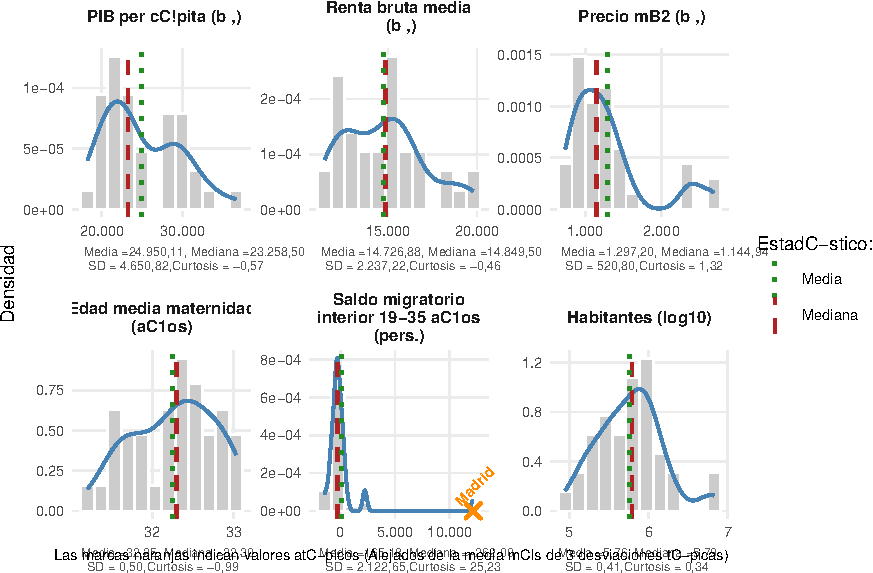
\includegraphics[width=1\linewidth]{ProyectoAED_files/figure-latex/histograma-1} \end{center}

En los histogramas observamos la media y la mediana de cada variable,
así como los valores atípicos según la regla de la desviación típica. La
edad media de maternidad, la renta bruta media y el logaritmo de la
población son las variables más próximas a la simetría (media y mediana
casi coinciden), mientras que el PIB per cápita y el precio del metro
cuadrado presentan asimetría positiva, con la media por encima de la
mediana por la cola de provincias de renta y precios altos. El caso más
extremo es el del saldo migratorio: su media es nula (como cabe esperar
al tratarse de saldos netos entre provincias) pero su mediana es
negativa (-308 personas), es decir, la mayoría de provincias pierde
población joven y Madrid, único valor atípico según este criterio,
concentra las ganancias, lo que explica en buena medida una curtosis de
33,16.

Para complementar el análisis, representamos también diagramas de caja y
detectamos los valores atípicos usando la regla del rango
intercuartílico.

\begin{figure}[H]

{\centering 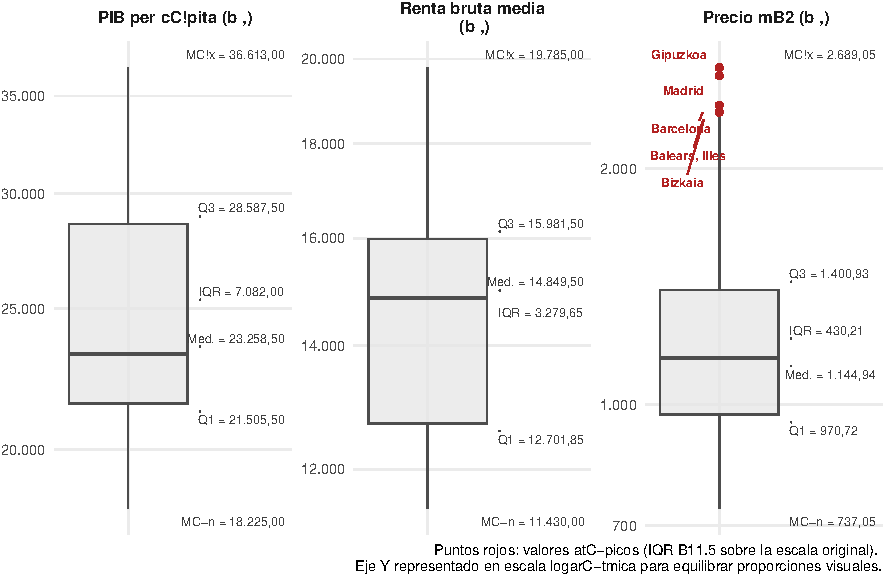
\includegraphics[width=1\linewidth]{ProyectoAED_files/figure-latex/boxplots-1} 

}

\caption{Distribuci<U+00F3>n de las variables socioecon<U+00F3>micas.}\label{fig:boxplots-1}
\end{figure}
\begin{figure}[H]

{\centering 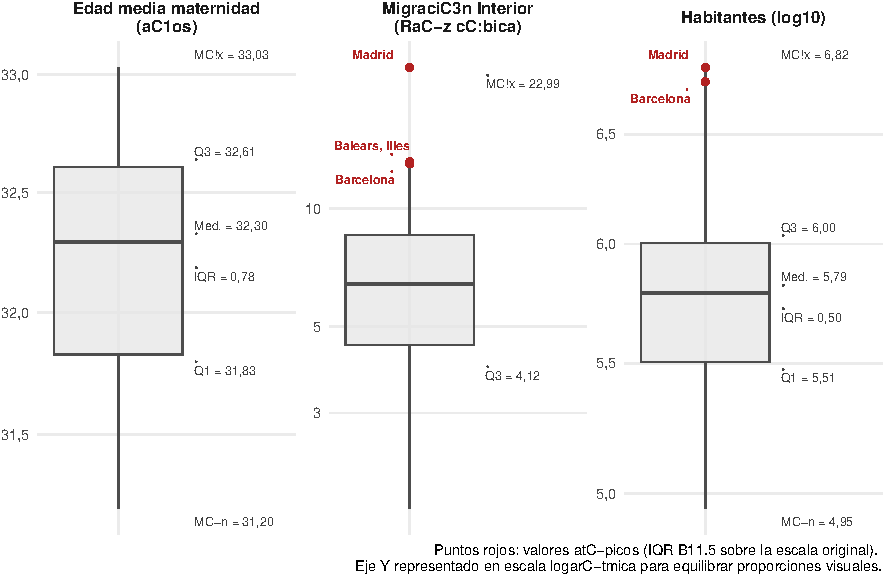
\includegraphics[width=1\linewidth]{ProyectoAED_files/figure-latex/boxplots-2} 

}

\caption{Distribuci<U+00F3>n de las variables socioecon<U+00F3>micas.}\label{fig:boxplots-2}
\end{figure}

Con el criterio del rango intercuartílico aparecen más valores atípicos
que con la regla de las tres desviaciones, al ser un criterio más
sensible a las colas. El precio del metro cuadrado destaca por varios
atípicos por encima del bigote superior. En la migración interior
destacan Madrid, Illes Balears y Barcelona como receptoras y Jaén como
la provincia con mayor pérdida. El análisis incluye únicamente las 50
provincias, por lo que Ceuta y Melilla no forman parte de esta
comparación.

Para visualizar la distribución de las variables laborales, hacemos uso
de diagramas de cajas para comparar por sector cada una de las
variables.

\begin{Shaded}
\begin{Highlighting}[]
\FunctionTok{boxplot\_laborales}\NormalTok{(panel\_analisis\_2019)}
\end{Highlighting}
\end{Shaded}

\begin{center}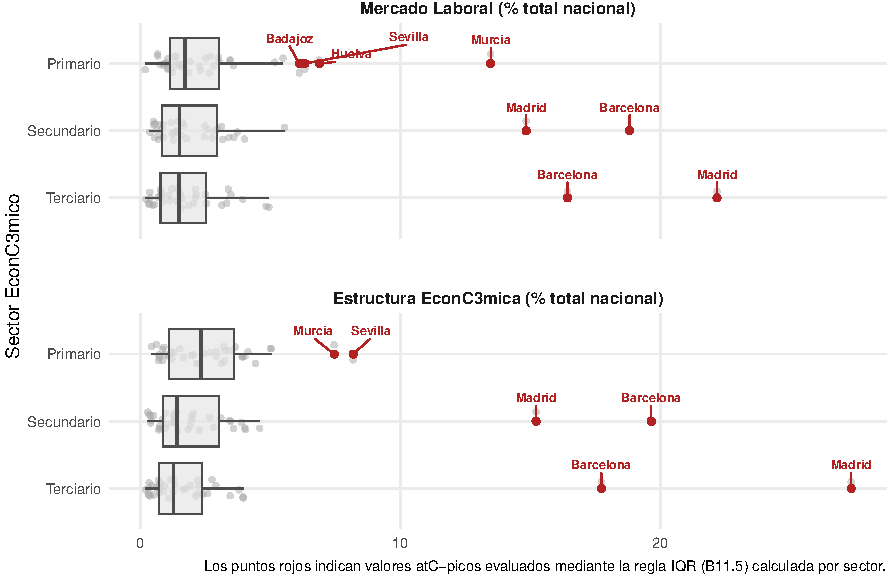
\includegraphics[width=1\linewidth]{ProyectoAED_files/figure-latex/unnamed-chunk-8-1} \end{center}

Podemos observar de nuevo datos muy heterogéneos y valores extremos muy
altos. En los sectores secundario y terciario los atípicos son siempre
las mismas provincias de gran tamaño (Madrid, Barcelona y
Valencia/València), que concentran una parte desproporcionada del empleo
y del valor añadido nacional (Madrid supera el 20 \% del VAB terciario),
mientras que en el sector primario destacan Almería y Murcia en empleo,
y Sevilla y Almería en VAB.

\subsection{Análisis Bivariante y
Multivariante}\label{anuxe1lisis-bivariante-y-multivariante}

Una vez constatada la heteoregeidad de los datos en el análisis
univariante, en esta sección buscamos cruzar las variables para dar
respuesta a las preguntas planteadas en la introducción. Para sintetizar
las múltiples interacciones entre distintas variables, hacemos uso de la
matriz de correlación. Como hemos visto en el análisis univariante, las
distribuciones presentan asimetrías, colas pesadas, y en varios casos
outliers. Para que esto no afecte de manera significativa a las
correlaciones, en algunos casos usaremos medidas derivadas de los datos.

\begin{enumerate}
\def\labelenumi{\arabic{enumi}.}
\item
  La densidad de población en lugar del número de habitantes,es decir
  \[Densidad\_Pobl. = \frac{Num\_Habitantes}{Superficie\_Provincia}.\]
\item
  El esfuerzo de compra la vivienda, caclulada como el número de años de
  renta bruta media que se requieren para alcanzar el valor de una casa
  de \(90 m^2\).
  \[Esf\_Vivienda = \frac{90*Precio~m^2}{Renta~Bruta~Media}.\]
\item
  La brecha renta/PIB. Es decir, la magnitud de la renta bruta media con
  respecto al PIB per cápita.
  \[Brecha~ Renta/PIB = \frac{Renta~Bruta~Media}{PIB~per~capita}.\]
\item
  La migración joven por cada 1.000 habitantes:
  \[Mig\_Joven = \frac{Migracion\_Interior}{Num\_Habitantes}\cdot 1000.\]
\end{enumerate}

Usamos la correlación de Spearman, ya que al aplicar estas
transformaciones no lineales, la correlación de Pearson se distorsiona.

\begin{Shaded}
\begin{Highlighting}[]
\NormalTok{panel\_bivariante\_2019 }\OtherTok{\textless{}{-}} \FunctionTok{crear\_panel\_bivariante}\NormalTok{(panel\_analisis\_2019)}
\end{Highlighting}
\end{Shaded}

\begin{Shaded}
\begin{Highlighting}[]
\NormalTok{correlacion\_global }\OtherTok{\textless{}{-}} \FunctionTok{calcular\_matriz\_correlacion}\NormalTok{(}
\NormalTok{  panel\_bivariante\_2019, variables\_cluster, nombres\_variables\_cluster}
\NormalTok{)}
\NormalTok{matriz\_cor }\OtherTok{\textless{}{-}}\NormalTok{ correlacion\_global}\SpecialCharTok{$}\NormalTok{matriz}
\NormalTok{orden\_variables\_cor }\OtherTok{\textless{}{-}}\NormalTok{ correlacion\_global}\SpecialCharTok{$}\NormalTok{orden}
\FunctionTok{graficar\_matriz\_correlacion}\NormalTok{(matriz\_cor)}
\end{Highlighting}
\end{Shaded}

\begin{center}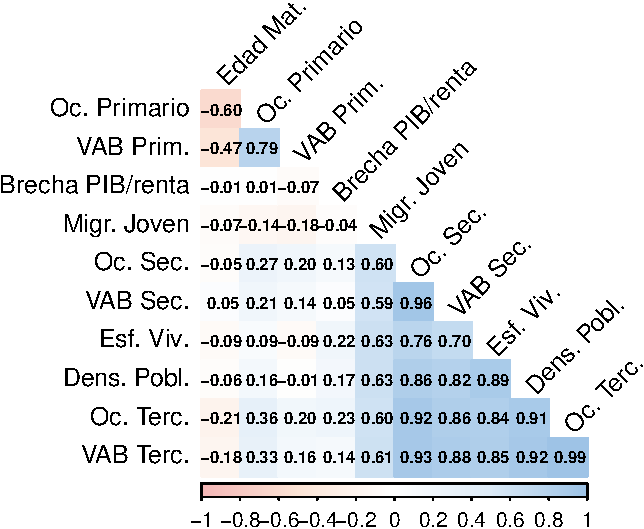
\includegraphics[width=1\linewidth]{ProyectoAED_files/figure-latex/unnamed-chunk-9-1} \end{center}

Observamos valores de correlaciones muy variados, algunos esperados como
la correlación entre el porcentaje de ocupación el VAB en cada uno de
los sectores. Hay otros que llaman la atención, como la correlación
entre la densidad de población y el esfuerzo de acceso a la vivienda.
Sin embargo, ninguno es tan alto como para asegurar una relación fuerte
entre dos variables. Como hemos visto en el análisis univariante de los
datos, tenemos datos muy heterogéneos con valores extremos, y
distribuciones asimétricas. Para responder a la pregunta sobre si las
relaciones entre los distintos indicadores ocurren de manera homogénea,
realizamos un agrupamiento de las provincias para separarlas en 4 grupos
(clustering jerárquico) con características socioeconómicas similares,
para observar si cambian las dinámicas entre estas, o por el contratio
no se alteran. En el siguiente mapa podemos observar un mapa con las
provincias divididas en los grupos correspondientes.

\begin{center}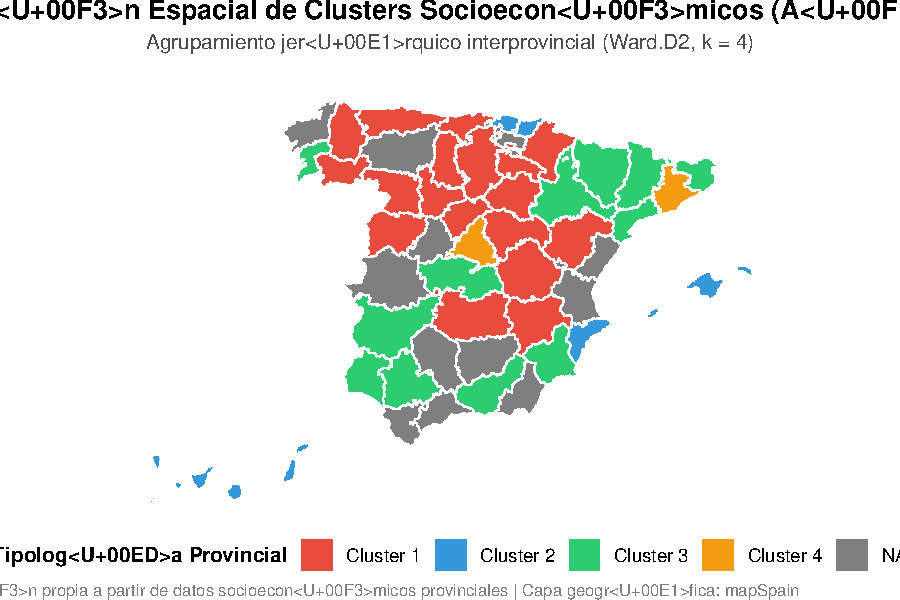
\includegraphics[width=1\linewidth]{ProyectoAED_files/figure-latex/unnamed-chunk-11-1} \end{center}

Por el mapa nos podemos hacer una idea de las características por las
que se ha formado cada grupo. Calculamos los valores promedios de cada
variable por grupo para observar las características de cada grupo.

\begin{table}[!h]
\centering
\caption{\label{tab:unnamed-chunk-12}Perfil socioecon<U+00F3>mico por Cluster}
\centering
\resizebox{\ifdim\width>\linewidth\linewidth\else\width\fi}{!}{
\begin{tabular}[t]{lrrrrrr}
\toprule
Cluster & Num\_Provincias & brecha\_pib\_renta & esfuerzo\_vivienda & Edad\_Media\_Maternidad & mig\_joven\_1000 & Densidad\\
\midrule
Cluster 1 & 18 & 0.61 & 6.31 & 32.47 & -1.15 & 37.98\\
Cluster 2 & 6 & 0.62 & 11.25 & 32.16 & 0.40 & 352.34\\
Cluster 3 & 12 & 0.58 & 7.60 & 31.88 & -0.42 & 87.10\\
Cluster 4 & 2 & 0.55 & 12.00 & 32.75 & 1.11 & 782.32\\
\bottomrule
\end{tabular}}
\end{table}

\begin{table}[!h]
\centering
\caption{\label{tab:unnamed-chunk-12}Perfil de estructura productiva por Cluster }
\centering
\resizebox{\ifdim\width>\linewidth\linewidth\else\width\fi}{!}{
\begin{tabular}[t]{lrrrrrrr}
\toprule
Cluster & Num\_Provincias & pct\_Ocupadas\_Primario & pct\_Ocupadas\_Secundario & pct\_Ocupadas\_Terciario & pct\_VAB\_Primario & pct\_VAB\_Secundario & pct\_VAB\_Terciario\\
\midrule
Cluster 1 & 18 & 1.56 & 1.14 & 0.87 & 1.98 & 1.19 & 0.77\\
Cluster 2 & 6 & 2.02 & 2.95 & 3.41 & 1.32 & 2.70 & 3.11\\
Cluster 3 & 12 & 4.78 & 2.35 & 2.10 & 4.30 & 2.30 & 1.86\\
Cluster 4 & 2 & 1.23 & 16.83 & 19.31 & 2.42 & 17.44 & 22.54\\
\bottomrule
\end{tabular}}
\end{table}

Podemos decir, que tenemos 4 clusters con perfiles diferentes, en los
que destacan:

\begin{enumerate}
\def\labelenumi{\arabic{enumi}.}
\item
  El primer cluster está formado por provincias con baja densidad, que
  no destacan en ningún sector en particular, que no aportan de manera
  significativa al total nacional, y de las que muchos jóvenes se van.
\item
  El segundo cluster está formado por provincias que tienen bastante más
  densidad, que Tampoco destacan en ningún sector, pero aportan más al
  total nacional que las del primer cluster.
\item
  El tercer cluster está formado por provincias con una densidad
  intermedia, y especialmente dedicadas al sector primario.
\item
  El cuarto cluster lo forman las provincias con áreas urbanas muy
  densas que reciben grandes cantidades de jóvenes de las otras partes
  del país, y concentran una parte importante de la actividad y el valor
  añadido de los sectores secundario y terciario.
\end{enumerate}

Por último, calculamos las correlaciones por cluster, para determinar si
las relaciones son heterogéneas o no.

\begin{Shaded}
\begin{Highlighting}[]
\NormalTok{df\_correlaciones }\OtherTok{\textless{}{-}} \FunctionTok{preparar\_correlaciones\_por\_cluster}\NormalTok{(}
\NormalTok{  panel\_bivariante\_2019,}
\NormalTok{  variables\_cluster,}
\NormalTok{  nombres\_variables\_cluster,}
\NormalTok{  orden\_variables\_cor}
\NormalTok{)}
\FunctionTok{graficar\_correlaciones\_por\_cluster}\NormalTok{(df\_correlaciones)}
\end{Highlighting}
\end{Shaded}

\begin{center}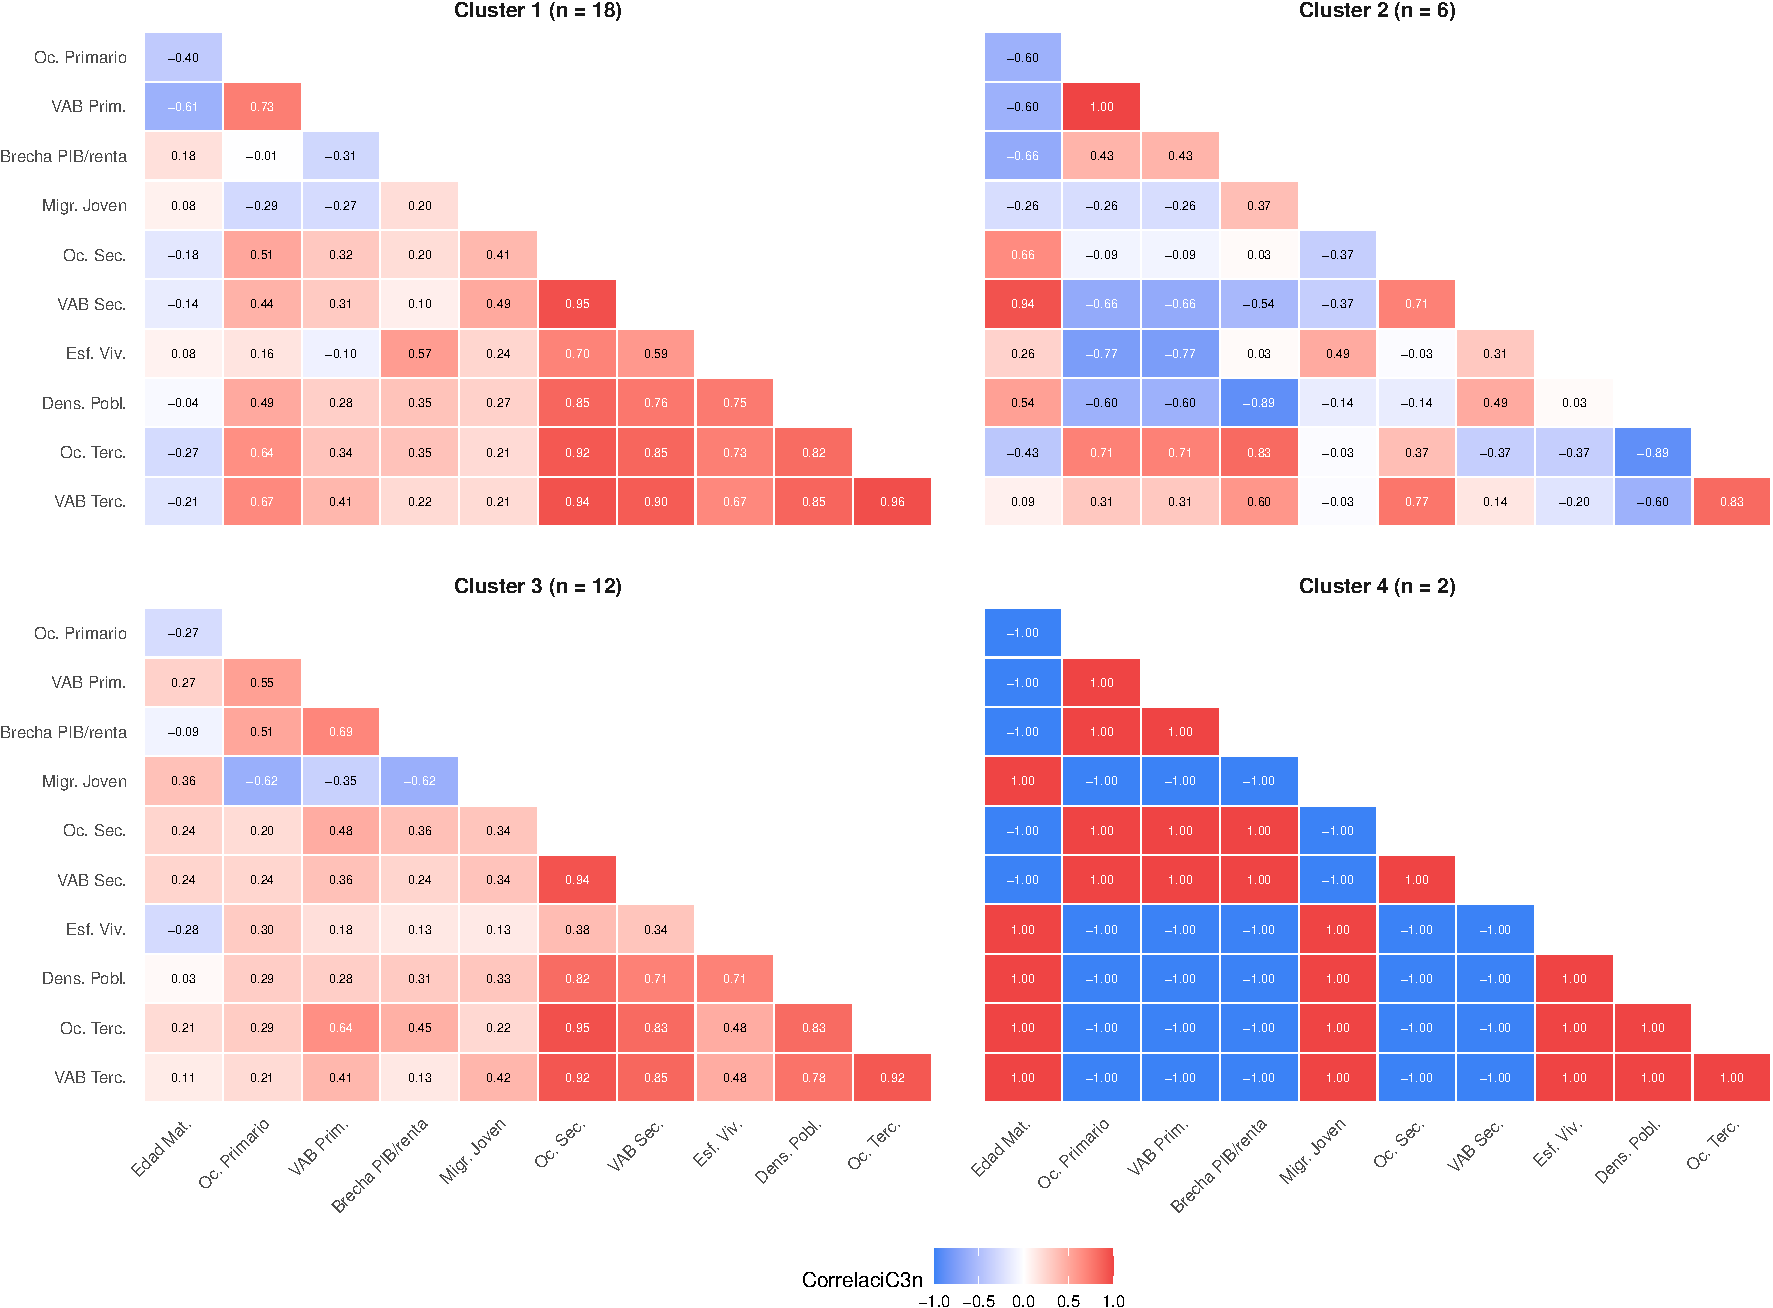
\includegraphics[width=1\linewidth]{ProyectoAED_files/figure-latex/correlaciones-por-cluster-1} \end{center}

Estas nuevas matrices de correlación poco tienen que ver con la
original. Observamos que la mayoría de valores cambian. En los grupos 3
y 4 al estar formados por dos elementos la correlación entre dos de sus
variables cualesquiera será 1 o -1 siempre, por lo que cualquier
interpretación que se haga sobre estos valores debe cogerse con pinzas.
Aún así, haciendo uso de las matrices de correlación de los dos primeros
clusters podemos dar respuesta a la pregunta, y afirmar que las
relaciones entre los distintos indicadores socioeconómicos no son
homogéneas a lo largo del país. Por ejemplo, podemos descatar que en el
primer cluster la brecha renta/PIB contribuye positivamente a la edad de
maternidad, mientras que en el segundo la relación es inversa.

\section{Conclusiones Finales}\label{conclusiones-finales}

El análisis provincial de España (2019) revela que la relación entre
estructura productiva e indicadores socioeconómicos es heterogénea. La
matriz global oculta realidades territoriales distintas que exigen
dividir el país en grupos en los que las dinámicas socioeconómicas son
similares, para poder responder preguntas más profundas sobre estas.
Destacan tres hallazgos clave:

1. Peso de los valores atípicos: Una minoría de provincias (Madrid,
Barcelona, País Vasco) concentra los máximos demográficos y económicos,
distorsionando las medias nacionales.

2. Vivienda vs.~Migración: El esfuerzo inmobiliario crece drásticamente
con la densidad poblacional (correlación 0,87). Pese a esta barrera,
solo los grandes núcleos (Clúster 4: Madrid y Barcelona) logran atraer
migración joven.

3. Estabilidad demográfica: La edad media de maternidad es la variable
más homogénea del país y la menos condicionada por la estructura
productiva.

Estas asociaciones no causales reflejan en gran medida el tamaño
absoluto de las provincias. Para futuros estudios, se sugiere medir la
estructura productiva a nivel interno (para evitar sesgos de tamaño) y
ampliar el análisis al periodo 2015-2021.

%%%%%%%%%%%%%%%%%%%%%%%%%%%%%%%%%%%%%%%%%%

\vspace{6pt}

%%%%%%%%%%%%%%%%%%%%%%%%%%%%%%%%%%%%%%%%%%
%% optional

% Only for the journal Methods and Protocols:
% If you wish to submit a video article, please do so with any other supplementary material.
% \supplementary{The following supporting information can be downloaded at: \linksupplementary{s1}, Figure S1: title; Table S1: title; Video S1: title. A supporting video article is available at doi: link.}

%%%%%%%%%%%%%%%%%%%%%%%%%%%%%%%%%%%%%%%%%%







%%%%%%%%%%%%%%%%%%%%%%%%%%%%%%%%%%%%%%%%%%
%% Optional

%% Only for journal Encyclopedia


%%%%%%%%%%%%%%%%%%%%%%%%%%%%%%%%%%%%%%%%%%
%% Optional
%%%%%%%%%%%%%%%%%%%%%%%%%%%%%%%%%%%%%%%%%%
\begin{adjustwidth}{-\extralength}{0cm}

%\printendnotes[custom] % Un-comment to print a list of endnotes



% If authors have biography, please use the format below
%\section*{Short Biography of Authors}
%\bio
%{\raisebox{-0.35cm}{\includegraphics[width=3.5cm,height=5.3cm,clip,keepaspectratio]{Definitions/author1.pdf}}}
%{\textbf{Firstname Lastname} Biography of first author}
%
%\bio
%{\raisebox{-0.35cm}{\includegraphics[width=3.5cm,height=5.3cm,clip,keepaspectratio]{Definitions/author2.jpg}}}
%{\textbf{Firstname Lastname} Biography of second author}

%%%%%%%%%%%%%%%%%%%%%%%%%%%%%%%%%%%%%%%%%%
%% for journal Sci
%\reviewreports{\\
%Reviewer 1 comments and authors’ response\\
%Reviewer 2 comments and authors’ response\\
%Reviewer 3 comments and authors’ response
%}
%%%%%%%%%%%%%%%%%%%%%%%%%%%%%%%%%%%%%%%%%%
\PublishersNote{}
\end{adjustwidth}


\end{document}
